\newpage
\hypertarget{treeToModel vis}{}
\subsection{The visual transformation rules}
\visHeader

As a quick note before you start, remember that we have assumed a basic understanding of TGGs and the different ways of using EA productively to create rules.
If you find this section challenging, we recommend first working through Part IV to cover TGG fundamentals.

\begin{itemize}

\subsubsection{FolderToLibraryRule} % ---------------------------------

\item[$\blacktriangleright$] Return to your open project in EA and expand the \texttt{<<Rules Package>>}, then open the \texttt{Rules} diagram.
Create a new rule named \texttt{Fol\-der\-To\-Lib\-rar\-y\-Rule} and double-click its element to open the rule diagram. Complete it as depicted in
Fig.~\ref{ea:FolderIntoLibrary_Complete}.

\vspace{0.5cm}

\begin{figure}[htbp]
\begin{center}
  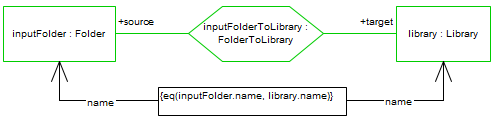
\includegraphics[width=\textwidth]{ea_FolderToLibraryRule}
  \caption{\texttt{FolderToLibraryRule}}
  \label{ea:FolderIntoLibrary_Complete}
\end{center}
\end{figure}

\item[$\blacktriangleright$] This is a simple rule that creates and connects equivalent \texttt{Folder} and \texttt{Library} instances. We're able to use this
entire rule as context for the next rule, which will handle the creation of shelves. Select \texttt{inputFolder}, \texttt{in\-put\-Fol\-der\-To\-Lib\-rary,} and
\texttt{library}, then use the eMoflon control panel to \texttt{derive} a new rule (Fig.~\ref{ea:controlPanel}).
Name this \texttt{ForAllShelfRule}.

\vspace{0.5cm}

\begin{figure}[htbp]
\begin{center}
  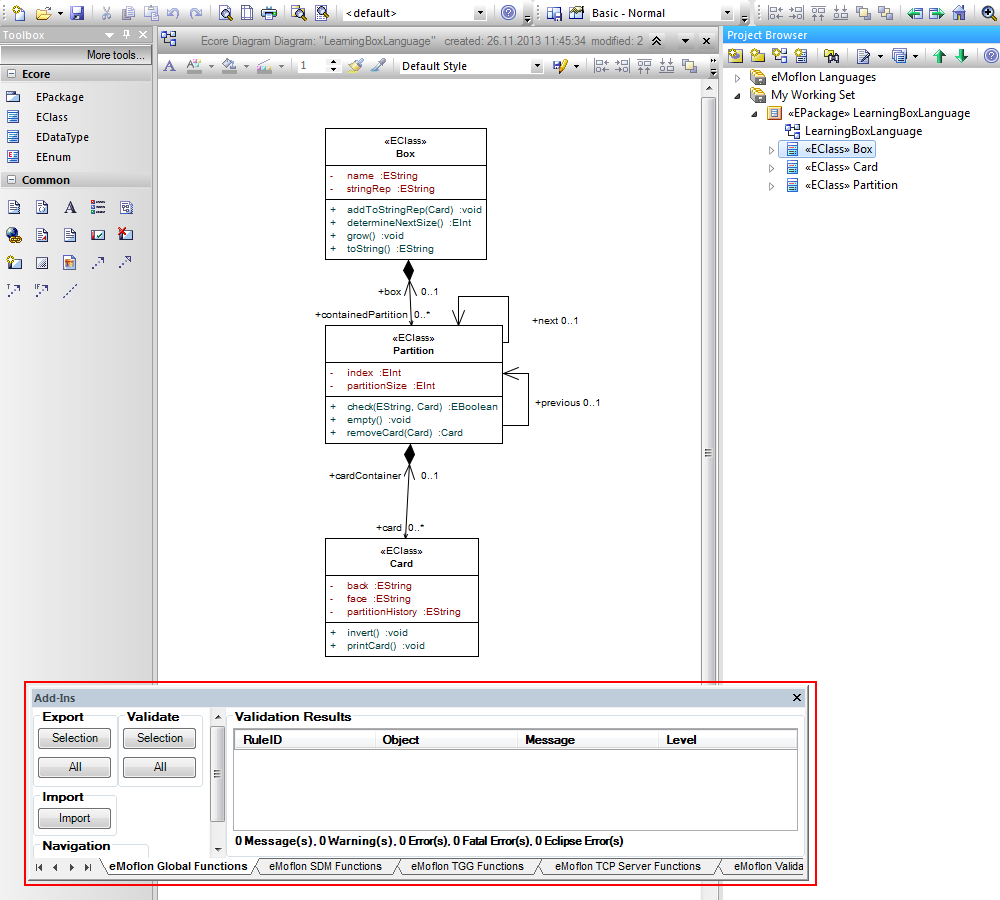
\includegraphics[width=\textwidth]{ea_controlPanel}
  \caption{Deriving a new rule with eMoflon's control panel}
  \label{ea:controlPanel}
\end{center}
\end{figure}

\newpage

\subsubsection{ForAllShelfRule} % ---------------------------------

The derivation procedure will open a new diagram with context elements from the first rule. This new rule is similar to
\texttt{Fold\-er\-To\-Lib\-rar\-y\-Rule}, except that it will connect new (green) elements to existing (black) containers. 

\item[$\blacktriangleright$] Complete the rule as depicted in Fig.~\ref{ea:ForAllShelves_Complete}. You'll need to create a new \texttt{FolderToShelf}
correspondence type in either the schema (as we did in the beginning), or on-the-fly by selecting \texttt{Create New Correspondence Type} in the quick-link
dialogue (Fig.~\ref{ea:corrOnTheFly}).

\begin{figure}[htbp]
\begin{center}
  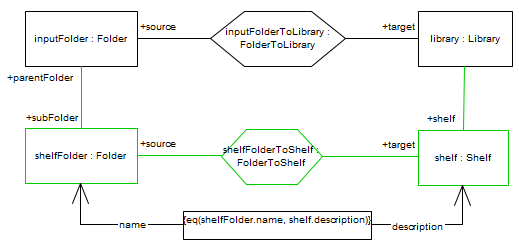
\includegraphics[width=0.9\textwidth]{ea_ForAllShelfRule}
  \caption{\texttt{ForAllShelfRule}}
  \label{ea:ForAllShelves_Complete}
\end{center}
\end{figure}

\begin{figure}[htbp]
\begin{center}
  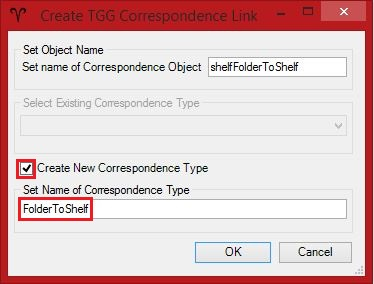
\includegraphics[width=0.6\textwidth]{ea_createNewLink}
  \caption{Creating a \texttt{FolderToShelf} correspondence type on-the-fly}
  \label{ea:corrOnTheFly}
\end{center}
\end{figure}

\subsubsection{NodeToDictionaryRule} % ---------------------------------

\item[$\blacktriangleright$] With the container \texttt{shelf} now assumed to exist, we are ready to handle dictionary \texttt{File} elements.
Analogously to how you began the previous rule, select \texttt{shelfFolder}, \texttt{shelfFolderToShelf}, and \texttt{shelf}, and derive
\texttt{NodeToDictionaryRule} with this context.

\vspace{0.5cm}

\item[$\blacktriangleright$] Complete it as depicted in Fig.~\ref{ea:NodeToDictionary_Complete}. As you can see, this rule creates a 
\texttt{dictionaryNode} and and its equivalent \texttt{dictionary}, and handles the first node in the tree structure. Nearly every
element is used to correctly set the \texttt{dictionary} and \texttt{dictionaryFile} names in two constraints.

\vspace{0.5cm}

\begin{figure}[htbp]
  \hspace{-0.7cm}
  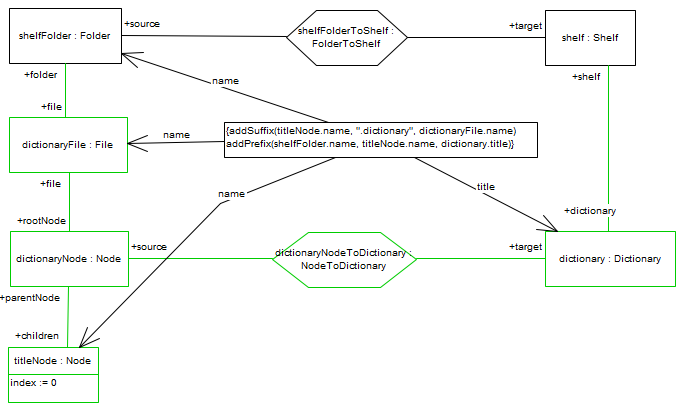
\includegraphics[width=1.2\textwidth]{ea_NodeToDictionaryRule}
  \caption{\texttt{NodeToDictionaryRule}}
  \label{ea:NodeToDictionary_Complete}
\end{figure}

\vspace{0.5cm}

\item[$\blacktriangleright$] Please note that the attribute constraint in \texttt{titleNode} is required in order to ensure that the node
with the title information is always the first child in the tree (index = 0). 

\newpage

\item[$\blacktriangleright$] Note that we could have also included another \texttt{node} here to handle the author, along with a third, fourth, or even
tenth \texttt{node} for a dictionary's entries, but that would mean the pattern would absolutely have to match to a single author and ten entry elements, which
may not always exist. Instead, we'll create separate rules for each of these which can be called as many (or as few) times as necessary.

\subsubsection{ForAllEntryRule} % ---------------------------------

\item[$\blacktriangleright$] Let's handle \texttt{entry node}s first. Create and complete \texttt{For\-All\-Ent\-ry\-Rule} as depicted in
Fig.~\ref{ea:ForAllEntry_Complete}. 

\vspace{0.5cm}

\begin{figure}[htbp]
\hspace{-0.5cm}
  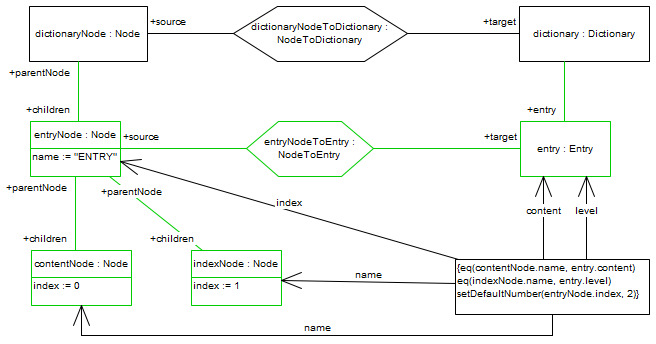
\includegraphics[width=1.1\textwidth]{ea_ForAllEntryRule}
  \caption{\texttt{ForAllEntryRule}}
  \label{ea:ForAllEntry_Complete}
\end{figure}

You can see that for every \texttt{entryNode}, \texttt{contentNode} and \texttt{indexNode} child elements are also created. When transforming from a tree to
dictionary, these are identified by their 0 and 1 indices. As such, the rule's first two constraints are used to ensure that this information is not
lost, guaranteeing their correct positions in the tree when transforming back.

\vspace{0.5cm}

The final constraint however, is one we haven't used before. If you re-examine your source \texttt{tree.xmi} model, you'll notice that every entry has a
different \texttt{index} value. This prevented us from setting an attribute constraint on \texttt{entryNode} but, as long as its index wasn't 0 indicating a
\texttt{titleNode} (as constrained in the previous \texttt{NodeToDictionaryRule}), it didn't matter. Unfortunately, this missing information means any new
\texttt{entryNode}s created in the backward transformation have a default 0 index value, and \emph{could} be mistaken by the rule. By using
\texttt{setDefaultNumber}, we have declared that any created default \texttt{index} attributes must be set to 2.

\subsubsection{AuthorRule} % ---------------------------------

\item[$\blacktriangleright$] We want to create a rule to handle authors next, so double-click the anchor in the top left of the diagram to return to
\texttt{NodeToDictionaryRule}.

\item[$\blacktriangleright$] We can begin this rule by deriving from \texttt{DictionaryNode}, \texttt{dictionary}, and \texttt{shelf}, but we'll need to add a
fourth context element, \texttt{library}, in accordance with the \texttt{Dictionary} metamodel, where each \texttt{author} is connected to its \texttt{dictionary} and
the \texttt{library} instance. Derive and create \texttt{AuthorRule} as shown in Fig.~\ref{ea:AuthorRule}.

\vspace{0.5cm}

\begin{figure}[h]
  %\begin{centering}
  \hspace{-0.5cm}
  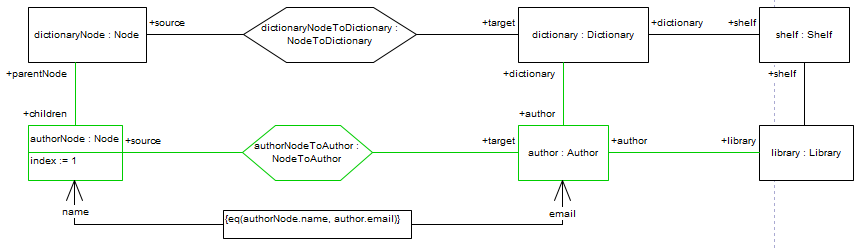
\includegraphics[width=1.1\textwidth]{ea_AuthorRule}
  \caption{\texttt{AuthorRule}}
  \label{ea:AuthorRule}
  %\end{centering}
\end{figure}

\end{itemize}

Handling all \texttt{author} instances however, can't be realised with a single rule. Here we have specified that, for every \texttt{authorNode} the rule
finds, an \texttt{author} instance should be created. This would be fine if we had unique authors for \emph{every} dictionary \texttt{File}, but if you take
look at both of the french \texttt{numbers} files, you'll notice they both have the same contact information. This means that our \texttt{Dictionary} will have
two identical \texttt{author} instances for one \texttt{library}.

Some users may be okay with this, and not care about redundant information so long as all the correct information is there, but others may prefer a
more concise structure. How can we refine this rule so that it's easy to handle both cases?

eMoflon's visual syntax has a cool \emph{refinement} feature which enables you to adjust specific elements in a rule, without having to redraw an entire
diagram exactly as before, save for one or two minor differences. Given that we want rules to handle either \emph{always} creating an \texttt{author}, or
checking for an existing one first, (both which will be identical to \texttt{AuthorRule} except for the binding and reference links on the matched
\texttt{authorNode}), this feature is exactly what we need.

\begin{itemize}

\item[$\blacktriangleright$] Return to the \texttt{Rules} diagram. Since we're no longer implementing \texttt{AuthorRule} directly, we need to make it
\texttt{abstract}. Select the rule, then hit \texttt{alt + enter} to open its properties dialogue.

\item[$\blacktriangleright$] Switch to the \texttt{Details} tab, and select \texttt{Abstract} from the list of properties (Fig.~\ref{ea:abstractDetails}). 
Affirm and close by pressing \texttt{OK}.

\vspace{0.5cm}

\begin{figure}[htbp]
\begin{center}
  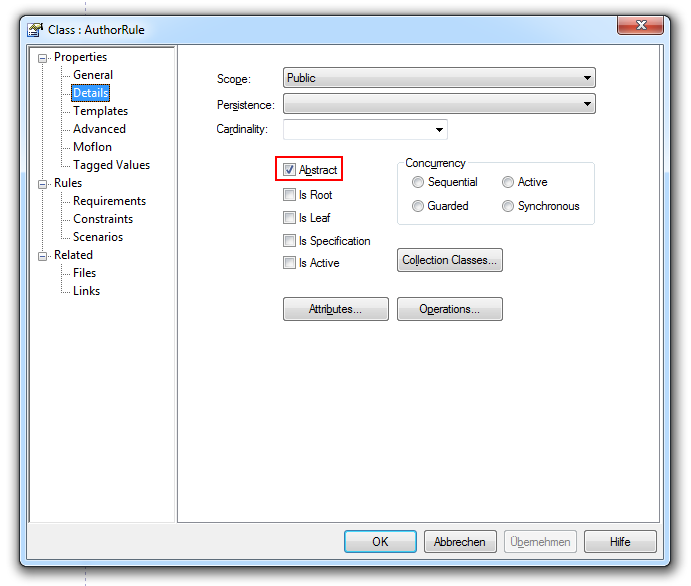
\includegraphics[width=\textwidth]{ea_abstractDetails}
  \caption{Declaring \texttt{AuthorRule} as abstract}
  \label{ea:abstractDetails}
\end{center}
\end{figure}

\end{itemize}

\newpage

Now we can develop our two rules. The key idea when building refinements is to imagine the new rules being placed directly over the pattern they inherit
from, similar to a transparency sheet. These rules will execute \texttt{AuthorRule} exactly, except for whatever modifications you make (which ``cover'' the
original element).

Let's make the rule that handles an already existing author first. Inspecting \texttt{AuthorRule}, we still want the rule to match a new \texttt{authorNode}
and create a link between \texttt{author} and \texttt{dictionary}, but the \texttt{author} element, and the link connecting it to \texttt{library} should
already exist, (i.e., be `black').

\begin{itemize}

\subsubsection{ExistingAuthorRule} % ---------------------------------

\item[$\blacktriangleright$] In \texttt{AuthorRule}'s diagram, select \texttt{authorNode} and \texttt{library}, and press \texttt{Derive}. Enter
\texttt{ExistingAuthorRule} as the rule's name but given that we want to refine the selected elements, not use them as context elements,
be sure to select the \texttt{exact copy} option (Fig.~\ref{ea:deriveRefinement}).

\begin{figure}[htbp]
\begin{center}
  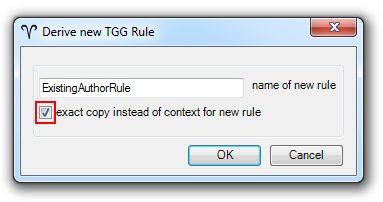
\includegraphics[width=0.6\textwidth]{ea_deriveRefinement}
  \caption{Deriving a refinement rule}
  \label{ea:deriveRefinement}
\end{center}
\end{figure}

\item[$\blacktriangleright$] The rule diagram will open in the editor, with the elements in the same place you copied them from. Complete the rule by changing
\texttt{author} and the link to \texttt{library} to \texttt{Check Only} as depicted in Fig.~\ref{ea:existingAuthorRule}.

\begin{figure}[htbp]
\begin{center}
  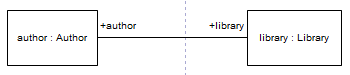
\includegraphics[width=0.7\textwidth]{ea_ExistingAuthorRule}
  \caption{\texttt{ExistingAuthorRule}}
  \label{ea:existingAuthorRule}
\end{center}
\end{figure}

\item[$\blacktriangleright$] If you're having difficulty visualising the entire rule with this minor modification, note that EA allows you to drag and drop all
elements from the basis rule as links so they're represented in the diagram. Figure~\ref{ea:existingAuthorRuleComplete} represents the entire
\texttt{ExistingAuthorRule}. This how the rule would have looked without using rule refinement.

\vspace{0.5cm}

\begin{figure}[htbp]
\begin{center}
  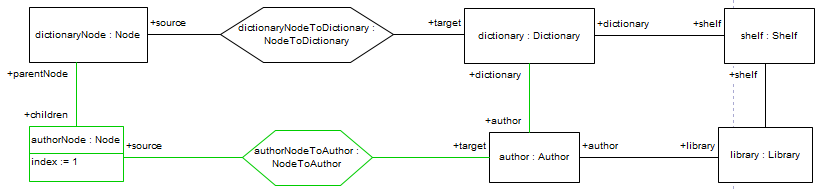
\includegraphics[width=\textwidth]{ea_ExistingAuthorRuleComplete}
  \caption{\texttt{ExistingAuthorRule} (flattened)}
  \label{ea:existingAuthorRuleComplete}
\end{center}
\end{figure}

\vspace{-0.5cm}

\subsubsection{NewAuthorRule} % ---------------------------------

\item[$\blacktriangleright$] Return to \texttt{AuthorRule} and derive another copy of \texttt{authorNode} and \texttt{library} into a rule called
\texttt{NewAuthorRule}. We'll explain why further in the next section, but for now just leave it as it is, and don't change anything. As we have defined
\texttt{AuthorRule} as abstract, we need this concrete rule to handle new authors. The diagram should come to resemble Fig.~\ref{ea:NewAuthorRule}.

\vspace{0.5cm}

\begin{figure}[htbp]
\begin{center}
  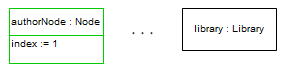
\includegraphics[width=0.6\textwidth]{ea_NewAuthorRule}
  \caption{Completed \texttt{NewAuthorRule}}
  \label{ea:NewAuthorRule}
\end{center}
\end{figure}

\item[$\blacktriangleright$] Of course, we could have left \texttt{AuthorRule} concrete and used just two rules, but having an explicit abstract rule, with
two concrete implementations of the possibilities, is clearer.

\item[$\blacktriangleright$] Return to the \texttt{Rules} diagram one last time. In order to ensure the new rules refine \texttt{AuthorRule},
quick-link from each to the root rule, choosing \texttt{Create Refinement Link} from the context menu. Your diagram should now resemble
Fig.~\ref{ea:refinementClasses}.

\item[$\blacktriangleright$] You're nearly done! Make sure everything is saved, and validate your TGG. 

\newpage

\vspace*{3cm}

\begin{figure}[htbp]
\begin{center}
  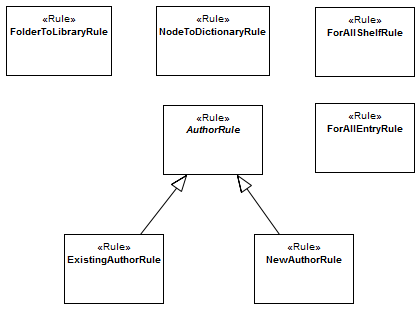
\includegraphics[width=0.8\textwidth]{ea_refinementLinks}
  \caption{Final \texttt{Rules} diagram}
  \label{ea:refinementClasses}
\end{center}
\end{figure}

%If a dialogue appears saying the attempt was
%unsuccessful, you may simply need to update the schema diagram which may not contain the new correspondence types you created on the fly. To do so, open the
%\texttt{DictionaryCodeAdapter} diagram, right-click anywhere in the window and add any missing elements by navigating to ``Insert Existing Element''
%(Fig.~\ref{ea:insertContext}). Selecting the missing correspondence types and the involved classes from the neccessary root package tree
% (Fig.~\ref{ea:insertTree}).

%\vspace{0.5cm}

%\begin{figure}[htbp]
%   \centering
%      \subfloat[Right-click to open the context menu]{
%        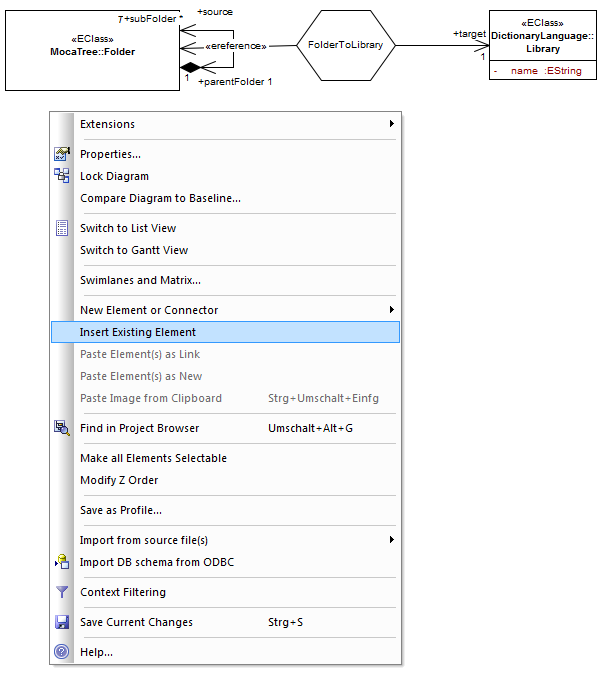
\includegraphics[width=0.7\textwidth]{ea_InsertExistingElements}
%        \label{ea:insertContext}
%      }
%      \\
%      \subfloat[Check your \texttt{TGG}, \texttt{DictionaryLanguage}, and \texttt{MocaTree} packages for elements.]{
%        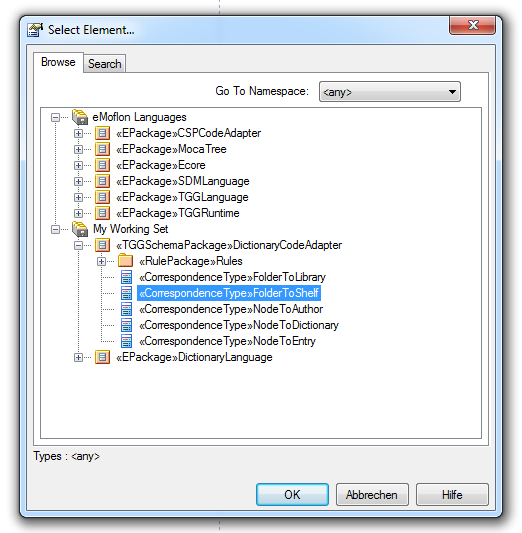
\includegraphics[width=0.7\textwidth]{ea_insertElementTree}
%        \label{ea:insertTree}
%      }
%\end{figure}

% \item[$\blacktriangleright$] Your schema diagram should resemble Fig.~\ref{ea:Schema_Complete} upon exit. Validate the project once again, then switch to the
% Eclipse workspace and refresh the package explorer.

% \newpage

% \vspace*{3cm}

% \begin{figure}[htbp]
%  \hspace{-1.5cm}
%  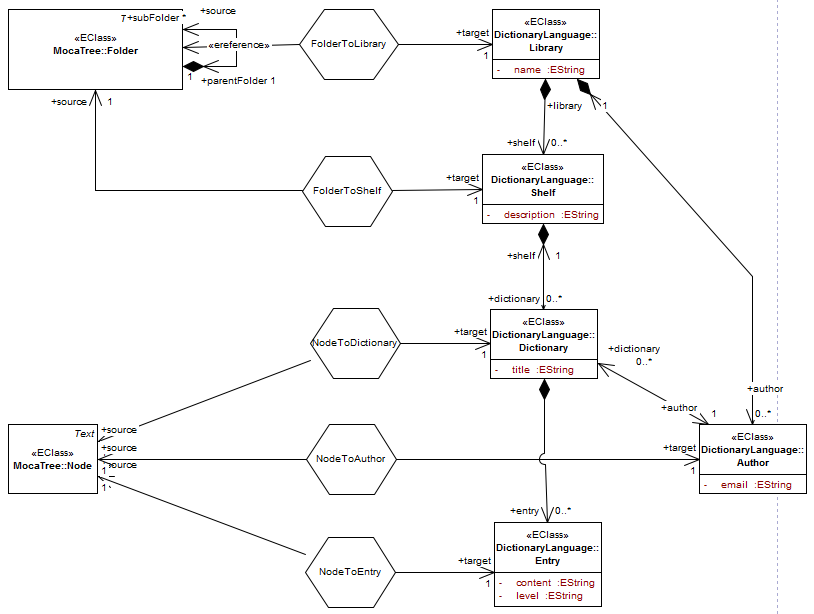
\includegraphics[width=1.3\textwidth]{ea_finalSchema}
%  \caption{The completed TGG Schema}
%  \label{ea:Schema_Complete}
%\end{figure}

\jumpSingle{t2m close}

\end{itemize}
